\documentclass[a4paper,10pt]{article}

%======================================================================
%	Bearbeitung sowohl mit LaTeX als auch mit pdfLaTeX ermoeglichen
%======================================================================
\usepackage{ifpdf}

%======================================================================
%	Verwendete Pakete
%======================================================================
% set language for sorting, hyphenation, sections etc.
\usepackage[ngerman,american]{babel}		% american ist default

%% Latex mit deutschen Umlauten:
%% http://www.cs.albany.edu/~herrmann/latex_umlaute/
%\usepackage[latin1]{inputenc}   % direkte Eingabe von ü,ö,ä,ß in Tex-Source-File erlaubt (statt "a, "o etc.)

\usepackage[utf8]{inputenc}

\usepackage[T1]{fontenc}				% EC-Schriften verwenden (vs. DC) da 8-Bit
				% EC-Schriften als T1-kodierten CM-Schriften
				% European/Ext.-Computer-Modern-(EC)-Schriften
				% Umlaute, Anführungszeichen ...
				% => Umlaute koennen von Latex richtig getrennt werden
				% FAQ 5.3.2
								
\usepackage{ae,aecompl}		% virtuelle-CM-Fonts
				% da EC nicht als PostScript-(Type-1) verfuegbar
				% => keine echten Umlaute in PDF-Dokumenten,
				% sondern nur ``a'' mit zwei Punkten als Extrazeichen drüber 
				%(Problem bei Suche im PDF Viewer).
				% Das ae-Package ermöglicht wieder die korrekte 
				% Suche.
				% By loading the ae package (\usepackage{ae}), 
				% you loose some characters as mentioned in 
				% README. 
				% The package aecompl by Denis Roegel restores
				% these characters which are taken from the ec 
				% fonts. If you use pdftex, you will get these 
				% characters as bitmaps, but this might be 
				% better than not having them at all.


%\usepackage{times, mathptm}	% TimesNewRoman Schrift (Acrobat Reader Fonts), 
				% dazu braucht man auch den entsprechenden 
				% Zeichensatz für den Math-Mode
%\usepackage{pslatex}		% ? mathematische Formeln mit Standard 
												% Postscript Fonts gesetzt
				% Paket     Roman         Serifenlos  Typewriter
				% -----------------------------------------------
				% times     Times         Helvetica   Courier
				% palatino  Palatino      Helvetica   Courier
				% newcent   NewCenturySch AvantGarde  Courier
				% bookman   Bookman       AvantGarde  Courier
				% Diese Schriften sind die Standard-PostScript-Schriften
				% und in jedem Drucker verfügbar

\usepackage{
%	german,			% Deutsche Trennungen (ALTE Rechtschreibung), 
							% Anführungsstriche und mehr 
%	ngerman,		% Deutsche Trennungen (NEUE Rechtschreibung), 
							% Anführungsstriche und mehr
							%
%	acronym,		% Verwaltung von Abkuerzungen
%	bibgerm,		% Deutsche Bibliographie, z.B. für package gerapali (German APA-like)
	calc,				% Erweiterung der arithmetischen Funktionen in LaTeX
							% wird verwendet um Titelseite zu zentrieren
	color,			% im Laufenden Text einfach mit \color{Farbe) zwischen den 
							% Farben umschalten, wobei Farbe einfach 
							% durch z.B. red, blue, black etc. ersetzt wird
							% \textcolor{farbe){Text)
%	epigraph,		% Zitat am Kapitelanfang
%	fancyhdr,		% Kopf- und Fußzeilen von Dokumenten frei 
							% gestalten (ähnlich scrpage2)
%	fancybox,		% shadowbox, doublebox, ovalbox, Ovalbox 
%	fancyvrb,		% verbatim Erweiterung:
	float,			% Positionierung von Gleitobjekten genau an der Stelle, wo man möchte
							% In der 'figure'- oder 'table'-Umgebung muss die 
							% Positionierung [H] gesetzt werden
%	glosstex,		% Glossar und Abkürzungsverzeichnis
%	mdwlist,		% compact list: itemize* ..
%	scrdate,		% \todaysname 
%	scrtime,		% \thistime
%	scrpage2,		% Kopf- und Fußzeilen flexibel gestalten
							%
%	moreverb,		% verbatim-ähnlich: boxedverbatim, listing
%	verbatim,		% Darstellung von "Text, wie er eingegeben wird"
							%
%	lscape,			% Erstellt eine um 90% gedrehte *neue* Seite
%	textcomp,		% Sonderzeichen
%	booktabs,		% Tabellenlinien
%	longtable,			% Tabellen > 1 Seite
%	supertabular,		% Tabellen > 1 Seite
%	tabularx,		% The tabularx package defines a tabular environment that generates a table with a specified width. The package automatically adjusts the widths of certain columns rather than adding space between columns. 
%	ltxtable,		% tabularx + longtable
%	multicol,		% mehrspaltige Zeilen
	multirow,		% mehrzeilige Spalten
	array,
	varioref,		% intelligent page references (``see figure 5 on page 7'', ``see figure 3.2 on the facing page''...)
%	endnotes,		% Fussnoten -> Endnoten
%	rotating,		% sidewaystable und sidewaysfigure
	natbib,			% natbib package for handling both author-year and numerical BibTeX styles
%	marvosym,		% Euro etc.
% wasysym			% various symbols
%	pstricks,		% replace text in eps figures by, e.g., math formulas
% picinpar,		% picture in paragraph: window-environment, tabwindow, figwindow etc.
	amsmath,		% AMS math package
	amsfonts,		% AMS math fonts
	amssymb,		% AMS symbols
%	amsthm,			% AMS theorem environments: http://www.math.ucsd.edu/~jeggers/latex/amsthdoc.pdf
%	amscd,			% very simple commutative diagrams (there are more powerful packages)
%	listings,		% source code listings
%	setspace,		% Durchschuss/Spacing
%	xspace,			% Define commands that appear not to eat spaces. 
}

% Für schöne Darstellung von Algorithmen
%\usepackage{algpseudocode}					% algorithmicx-package: programs in pseudocode (``algorithmic''-environment)
%\algrenewcommand\algorithmicforall{\textbf{for each}}

%\usepackage[config=altsf,lofdepth=2]{subfig}			% Figures broken into subfigures

%======================================================================
%		PDF <=> DVIPS
%======================================================================
\ifpdf
	\usepackage{thumbpdf}		% Thumbnails in PDF einbetten, dafür muss erst
					% eine .tpt-Datei erstellt werden (siehe Makefile)
	\usepackage{pdflscape}
	\usepackage[pdftex]{graphicx}

	\definecolor{darkblue}{rgb}{0,0,.5}

	\usepackage[
		pdftex=true, 						% pdftex output 
		breaklinks=true, 				% it's ok to introduce a linebreak into links (may break some older viewers)
		pdfpagelabels=true, 		% name pages, e.g.\ ``ii (4 of 40)'', to fix ``pdfTeX warning (ext4)'' problem
		plainpages=false,				% use named pages as page labels, to fix ``pdfTeX warning (ext4)'' problem
%		colorlinks=true,				% Achtung! Farbige Links werden mitgedruckt, farbige Rahmen nicht!
		linkcolor=darkblue,
		citecolor=darkblue,
		menucolor=darkblue,
%		pagecolor=darkblue,
		urlcolor=darkblue,
	]{hyperref}
% pagebackref 
% die hyperref-Erweiterungen fuer PDF
% Einstellungen in hyperref.cfg
% letzte Angabe der Präambel
% Paket definiert viele interne Kommandos um
	\pdfcompresslevel=9     	% compression level for text and image;
%	\DeclareGraphicsRule{*}{mps}{*}{}
\else
	\usepackage[dvips]{graphicx}
	\usepackage[dvips, colorlinks=false, pdfborder=0]{hyperref}		% die hyperref-Erweiterungen fuer PostScript
\fi


%======================================================================
%		.eps-Dateien in PDF-Files
%======================================================================
% Damit das klappt, muss pdflatex mit der Option 
% 	'-shell-escape' (teTex, TeX Live) oder
%   '--enable-write18' (MikTex)
% aufgerufen werden und alle Grafiken ohne Dateiendung in den
% '\includegraphics{}'-Kommandos stehen.
\ifpdf
%	\def\pdfshellescape{1}	
			% Simulieren, dass '--enable-write18' angegeben wurde,
			% um fehlerhafte ``epstopdf Warning'' abzuschalten
			
	\usepackage{epstopdf}
	\newcommand{\inputfig}[1]{\input{#1.pstex_t}}
	\DeclareGraphicsExtensions{.ps,.pstex,.eps,.pdf}
	\DeclareGraphicsRule{.pstex}{pdf}{.pdf}{`epstopdf #1}
	\DeclareGraphicsRule{.ps}{pdf}{.pdf}{`epstopdf #1}
\else
	\usepackage{epsfig}
	\newcommand{\inputfig}[1]{\input{#1.pstex_t}}
	\DeclareGraphicsExtensions{.pstex,.eps}
\fi

% \usepackage{pdfpages}		% include pages from another PDF document with \includepdf{} 
												% (must be loaded _after_ graphicx)


%======================================================================
%	kile inverse forward search
%======================================================================

\usepackage[active]{srcltx}


%======================================================================
%	user.sty
%======================================================================

\usepackage{user}	% Makros in user.sty 
			% \epsinc{bild.eps}{scale=1}{Bildunterschrift}
			% \missing{Beweis fehlt noch}
			% \comment{Ein Kommentar}
			

%======================================================================
%	Einstellungen
%======================================================================

\setcounter{tocdepth}{3}

% ---------------------------------------------------------------------
\graphicspath{{img/}}	% Angabe der Pfade, wo die Grafiken liegen; 
											% mehrere Pfade sind möglich
				
% ---------------------------------------------------------------------
\flushbottom			% Ausrichtung der Seitenenden jeweils auf 
									% gleicher Höhe

%opening
\title{Documentation of the GGP Rating System}
\author{Martin Günther}


%======================================================================
%	Makros
%======================================================================

% %\newcommand{\gdl}[1]{\mbox{\lstinline[style=gdl, columns=fullflexible]{#1}}}
% %\newcommand{\gdl}[1]{\mbox{\lstinline[style=gdl, columns=fixed]{#1}}}
% \newcommand{\gdl}[1]{\mbox{\ttfamily{#1}}}
% 
% %\newcommand{\goal}{\texttt{goal}}
% %\newcommand{\terminal}{\texttt{terminal}}
% \newcommand{\goal}{\gdl{goal}}
% \newcommand{\terminal}{\gdl{terminal}}
% 
% %\newcommand{\function}[1]{\operatorname{#1}}
% \newcommand{\function}[1]{\ensuremath{#1}}
% 
% \newcommand{\Holds}{\function{Holds}}
% \newcommand{\Poss}{\function{Poss}}
% \newcommand{\Do}{\function{Do}}
% \newcommand{\Stateof}{\function{State}}
% \newcommand{\Terminal}{\function{Terminal}}
% \newcommand{\Goal}{\function{Goal}}
% 
% %%% incredible in fluent falculus %%%
% \newcommand{\Stack}{\function{S}}
% \newcommand{\Unstack}{\function{U}}
% 
% \newcommand{\Clear}{\function{Clear}}
% \newcommand{\Table}{\function{Table}}
% \newcommand{\On}{\function{On}}
% \newcommand{\Succ}{\function{Succ}}
% 
% \newcommand{\Step}{\function{Step}}
% 
% \newcommand{\Move}{\function{Move}}
% \newcommand{\Grab}{\function{Grab}}
% \newcommand{\Drop}{\function{Drop}}
% 
% \newcommand{\Cell}{\function{Cell}}
% \newcommand{\Gold}{\function{Gold}}
% %%%%%%%%%%%%%%%%%%%%%%%%%%%%%%%%%%%%%%%
% 
% \newcommand{\foo}{\function{foo}}
% \newcommand{\foobar}{\function{foobar}}
% 
% 
% %%%%%%%%%%%%% Sorts %%%%%%%%%%%%%%%%%%%
% \newcommand{\sort}[1]{\textsc{#1}}
% 
% \newcommand{\ACTION}{\sort{Action}}
% \newcommand{\SIT}{\sort{Sit}}
% \newcommand{\FLUENT}{\sort{Fluent}}
% \newcommand{\STATE}{\sort{State}}
% %%%%%%%%%%%%%%%%%%%%%%%%%%%%%%%%%%%%%%%
% 
% 
% \newcommand{\stateupdate}{\function{state\_update}}
% \newcommand{\update}{\function{update}}
% 
% \newcommand{\subgameof}{\triangleleft}
% \newcommand{\nsubgameof}{\ntriangleleft}
% 
% 
% 
% \newcommand{\sigmahat}{{\hat{\sigma}}}
% \newcommand{\A}{{\mathcal{A}}}
% \newcommand{\F}{{\mathcal{F}}}
% \newcommand{\Scal}{{\mathcal{S}}}
% 
% % Note: semantically oriented dot commands
% % \dotsc for “dots with commas”
% % \dotsb for “dots with binary operators/relations”
% % \dotsm for “multiplication dots”
% % \dotsi for “dots with integrals”
% % \dotso for “other dots” (none of the above)
%  
% \newcommand{\eqdef}{\stackrel{\text{def}}{=}}
% \newcommand{\entails}{\models}
% 
% % \renewcommand{\implies}{\supset}
% 
% \newcommand{\game}[1]{\ensuremath{\langle \F_{#1}, \A_{#1} \rangle}}
% 
% % styles of the title page
% %\newcommand{\titlebasicstyle}{\rmfamily\upshape}
% \newcommand{\titlebasicstyle}{\sffamily\upshape}
% \newcommand{\titlestyleemph}[1]{\bf\large\titlebasicstyle {#1}}
% \newcommand{\titlestylesmall}[1]{\mdseries\large\titlebasicstyle {#1}}
% \newcommand{\titlestylemiddle}[1]{\mdseries\Large\titlebasicstyle {#1}}
% \newcommand{\titlestylelarge}[1]{\mdseries\LARGE\titlebasicstyle {#1}}
% 
% % neues Float ``mglisting''
% \floatstyle{ruled}
% \newfloat{mglisting}{tbp}{lom}[chapter]
% \floatname{mglisting}{Listing}
% \newcommand{\listlistingname}{List of Listings}
% \newcommand{\listoflistings}{\listof{mglisting}{\listlistingname}}
% 
% % Stil eines Funktionsnamens in Pseudocode, zur Verwendung im normalen Text
% \newcommand{\algfunction}[1]{\textsc{#1}}
% 
% % neues Float ``algorithm''
% \floatstyle{ruled}
% \newfloat{algorithm}{tbp}{loa}[chapter]
% \floatname{algorithm}{Algorithm}
% \newcommand{\listalgorithmname}{List of Algorithms}
% \newcommand{\listofalgorithms}{\listof{algorithm}{\listalgorithmname}}
% 
% 
% \newcommand{\bb}{\bar{b}}
% \newcommand{\bd}{\bar{d}}
	% Eigene Makros und Abkürzungen


\begin{document}

\maketitle

\begin{abstract}
This document describes the current implementation of the GGP rating system.
\end{abstract}

\section{Data structures}
First, some words on the used data structures (ref.\ table~\ref{tab:data_structures}).
The data structures used for player, game and match have the intuitive meaning, but there
is a new data structure called ``match set''. A match set simply is a collection of matches,
all played in the same year, round and day of a competition, and all on the same game.
All past competitions have featured such match sets, and explicit handling of match sets
makes it possible to process all matches of such a match set in one batch.

Another unusual entry is the  ``coefficients'' property of a game, which will be explained in section~\ref{sec:updating_game_information}. For now, it suffices to think of it as the information that the linear regression rating stores about a game.

\begin{table}
\begin{center}
\begin{tabular}{l m{2.8cm} m{6cm}}
\hline
\textbf{class} & \textbf{property} & \textbf{description} \\
\hline
player & rating & a single number reflecting the player's current rating (e.g.\ $1000.0$) \\ 
\hline
\multirow{3}{*}{game} & name & the game name (e.g.\ chess) \\ 
 & roles & the roles of the game (e.g.\ black, white) \\ 
 & coefficients &  linear-regression-specific game info \\
\hline
\multirow{7}{*}{match} & match ID & the ID of the match (e.g.\ Match.3390056123) \\ 
 & players & the participants of the match \textit{($\rightarrow$~player)} \\ 
 & scores & the scores ($0 \dotsc 100$) achieved by each player\\ 
 & match set & the match set that this match is part of \textit{($\rightarrow$~match set)} \\ 
\hline
\multirow{6}{*}{match set} & match set ID & the ID of this match set (e.g.\ MatchSet.385572910) \\ 
 & year, round, day, match set number & self-explanatory (e.g.\ 2007, 3, 2, 10) \\ 
 & game & the played game (by definition, this is identical for all played matches of a match set) \textit{($\rightarrow$~game)} \\
\hline
\end{tabular}
\end{center}
\caption{Data structures}
\label{tab:data_structures}
\end{table} 

\section{Linear regression rating}

The central idea of linear regression rating is summarized in an email by Jim Clune:
\begin{quotation}
Here's some notation:

\begin{tabular}{ll}
&\\
$g(m)$:    & game associated with match $m$ \\
$s(r, m)$: & score of role $r$ in match $m$ \\
$p(r, m)$: & player assigned to role $r$ in match $m$ \\
$q(p)$:    & rating of player $p$ \\
&
\end{tabular}

It seems to me that we want to be able to express $E[s(r, m)]$ (the
expected value of the score of role $r$ in match $m$) in terms of $q(p(r', m))$
for each role $r'$ in the game. One way to achieve this might be to assume
$E[s(r, m)]$ is a linear function of these variables and perfrom least-squares
linear regression. For a game with roles = $\{r_1, r_2, r_3\}$, this yields
relationships such as:

\[E[s(r_1, m)] = c_0 + c_1*q(p(r_1, m)) + c_2*q(p(r_2, m)) + c_3*q(p(r_3, m))\]

where $c_0, c_1, c_2, c_3$ are game-specific constants computed by the linear
regression.

We could then calculate the expected outcome for each player in a
given match and compare it with their actual outcome. If expected and
actual outcomes are the same, the rating remains unchanged.
Otherwise, the rating is adjusted up or down proportional to the
difference between the actual outcome and the expected outcome.

- Jim
\end{quotation}

The following sections will show how to update the game-specific coefficients $c_0, c_1, c_2, c_3$ (section~\ref{sec:updating_game_information}), how to calculate the expected scores of a player (section~\ref{sec:calculating_expected_scores}) and how to update the player ratings (section~\ref{sec:updating_player_ratings}).

\subsection{Updating the game information}
\label{sec:updating_game_information}

The linear regression rating algorithm keeps so-called ``game information'' about each played game. This game information is just a matrix of linear regression coefficients and reflects the relationship between the role a player plays, the ratings of all players in the game and the expected score of the player in a certain game.

As stated above, linear regression rating assumes that the expected score of a player playing role $r_1$ can be approximated by a linear function of the form:
\begin{equation}
	E[s(r_1, m)] = c_0 + c_1*q(p(r_1, m)) + c_2*q(p(r_2, m)) + c_3*q(p(r_3, m)) 
	\label{eqn:expected_performance}
\end{equation} 

The coefficients $c_0, \dotsc, c_3$ are updated immediately after each played match set for the whole batch of matches. (The coefficients are different for each role, so the game information for a 3-player game such as this would consist of $3 * 4 = 12$ coefficients.)

If, in a given match set, players with a high rating scored worse (on average) than players with a high rating, the coefficient associated with the target role ($c_1$ in the example above) can become negative. If this is the case, the linear regression is repeated without the target role, and the target role's coefficient is set to zero. There are no constraints on the other coefficients.

If there are already known coefficients from former matches, the weighted average of the old and new coefficients is stored.

\subsection{Calculating the expected scores}
\label{sec:calculating_expected_scores}
In the next step, the expected score of each player is calculated using formula~\ref{eqn:expected_performance}. If the calculated value is less than 0 or greater than 100, the actual expected value is set to 0 or 100, respectively. After that, the total expected scores of each player are calculated by summing up the player's expected scores in all matches that the player played in that match set, so that the total expected score can exceed 100.


\subsection{Updating the player ratings}
\label{sec:updating_player_ratings}

In a third step, the player rankings are updated according to the following formula:

\begin{equation}
 q'(p) \leftarrow q(p) + l * (a(p) - e(p))
\end{equation} 

where $q(p)$ and $q'(p)$ are the current and updated rating of player $p$, $l$ is the learning rate (cf.\ section~\ref{sec:constant_dynamic}), $a(p)$ is the actual and $e(p)$ the expected score. Update also takes place after each completed match set, so the player ratings are adjusted as quick as possible in order to provide more accurate information to the next game information updating step.

On a side remark, the player's ratings are initialized with a constant value ($1000$, at the moment).


\subsection{Constant vs.\ dynamic learning rate}
\label{sec:constant_dynamic}

The choice of the learning rate has a big impact on the actual results of the algorithm. If the learning rate is too large, the player ratings become erratic and don't converge. If the learning rate is too small, they take too long to converge. One solution is to use a dynamic learning rate: starting off with a high learning rate and reducing it over time.

\section{Results}

\subsection{Constant vs. Dynamic Learning Rate}
The results for one run of both algorithms are shown in figures \ref{fig:constant_linear_regression} and \ref{fig:dynamic_linear_regression}. Figure~\ref{fig:direct_scores} shows the actual scores for comparison.

\begin{figure}
 \centering
 \includegraphics[width=\textwidth]{constant_linear_regression_1_0}
 \caption{Linear regression ratings with a \textit{constant} learning rate (Competition 2007 Preliminaries, constant learning rate = 1.0)}
 \label{fig:constant_linear_regression}
\end{figure}

\begin{figure}
 \centering
 \includegraphics[width=\textwidth]{dynamic_linear_regression_60}
 \caption{Linear regression ratings with a \textit{dynamic} learning rate (Competition 2007 Preliminaries, dynamic learning rate = 6.0$\dotsc$1.6, linear descent)}
 \label{fig:dynamic_linear_regression}
\end{figure}

\begin{figure}
 \centering
 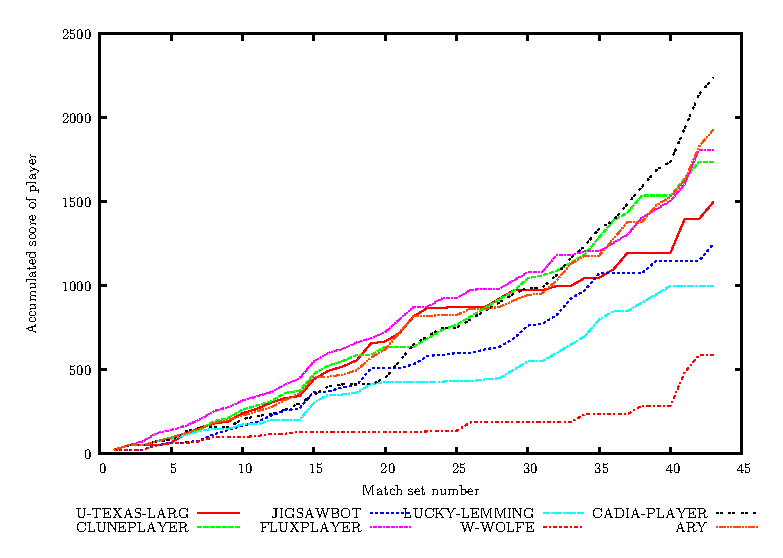
\includegraphics[width=\textwidth]{direct_scores}
 \caption{Weighted direct scores (Competition 2007 Preliminaries; using round weights 0.25, 0.5, 0.5 and 1.0)}
 \label{fig:direct_scores}
\end{figure}

\subsection{Re-Run}
As a quick ``sanity check'', both algorithms were re-run on the same data set, using the final player ratings to initialize the player ratings. The results are shown in figures \ref{fig:constant_linear_regression_with_initial_values} and \ref{fig:dynamic_linear_regression_with_initial_values}. As expected, the re-run produced results in the same range as the original one. The ratings are not constant, which can be partly explained by the fact that the players were under development during the competition, and so their playing strength did not remain constant. A good example is Cadia-Player, which performed moderately well during the first half of the competition, and so its rating is corrected downward during the re-run. In the second half of the competition, its playing strength greatly improved, and so the rating rises again.

\begin{figure}
 \centering
 \includegraphics[width=\textwidth]{constant_linear_regression_1_0_with_initial_values}
 \caption{Re-Run of linear regression ratings with a \textit{constant} learning rate}
 \label{fig:constant_linear_regression_with_initial_values}
\end{figure}

\begin{figure}
 \centering
 \includegraphics[width=\textwidth]{dynamic_linear_regression_60_with_initial_values}
 \caption{Re-Run of linear regression ratings with a \textit{dynamic} learning rate}
 \label{fig:dynamic_linear_regression_with_initial_values}
\end{figure}

\subsection{Calculated Weights}
To demonstrate the properties of the algorithm, some of the calculated weights will be analyzed.

The results of the 8 matches of tictactoe-large\footnote{Competition 2007 preliminaries, round 3, day 1 -- or short 2007-R3D1} are shown in table~\ref{tab:outcomes_tictactoelarge}. The first two columns are the ratings of both players, the third column shows the actual outcome and the last column contains the expected outcome, calculated via the coefficients in table~\ref{tab:coefficients_tictactoelarge}.

\begin{table}[htp]
	\begin{center}
		\begin{tabular}{rrrr}
			\hline
			\textbf{Rating 1} & \textbf{Rating 2} & \textbf{Outcome} & \textbf{Outcome (calc.)} \\ 
			\hline
			1455.0136    &	1166.2216    &	50.0         &	56.1203 \\
			1875.7368    &	1127.6833    &	100.0        &	65.8533 \\
			-729.6037    &	1519.9328    &	0.0          &	2.3262  \\
			2007.6933    &	837.7279     &	50.0         &	74.7947 \\
			1166.2216    &	1455.0136    &	50.0         &	43.8797 \\
			1127.6833    &	1875.7368    &	0.0          &	34.1467 \\
			1519.9328    &	-729.6037    &	100.0        &	97.6738 \\
			837.7279     &	2007.6933    &	50.0         &	25.2053 \\
			\hline
		\end{tabular}
	\end{center}
	\caption{Player ratings, real and predicted outcomes of tictactoe-large}
	\label{tab:outcomes_tictactoelarge}
\end{table}

\begin{table}[htp]
	\begin{center}
		\begin{tabular}{rrrr}
			\hline
			& \textbf{Best Estimate} & \textbf{SD} & \textbf{Coeff. [\%]} \\ 
			\hline
			$c_0$   &	50.000       &	26.5921      &	53.1841 \\
			$c_1$   &	0.0212       &	0.0129       &	60.8856 \\
			$c_2$   &	-0.0212      &	0.0129       &	-60.8856 \\
			\hline
		\end{tabular}
	\end{center}
	\caption{Coefficients for role 1 of tictactoe-large, $p = 0.0051$ (linear correlation coefficient probability)}
	\label{tab:coefficients_tictactoelarge}
\end{table}

Tictactoe-large is an example where the algorithm performs well. The prediction is statistically very significant ($p = 0.0051$), and the calculated weights are in the expected range. However, there are match sets which do not give satisfying results, like Amazons (2007-R4D1). Although the higher-rated player won in seven of the eight cases (table~\ref{tab:outcomes_amazons}), the algorithm assigns a negative coefficient to both roles (table~\ref{tab:coefficients_amazons}). The reason for this is probably that the difference in ratings is huge in the ``offending'' match (number 7). Since least-squares minimization is used, the linear regression algorithm prefers many smaller errors to one huge error and picks its coefficients accordingly. As already mentioned in section~\ref{sec:updating_game_information}, these results will not be used, and instead a linear regression without the target role will be performed.

\begin{table}[htp]
	\begin{center}
		\begin{tabular}{rrrr}
			\hline
			\textbf{Rating 1} & \textbf{Rating 2} & \textbf{Outcome} & \textbf{Outcome (calc.)} \\ 
			\hline
				1515.4385    &	710.5769     &	100.0        &	76.1431  \\
				1210.5041    &	2291.2757    &	0.0          &	22.6747  \\
				1939.6671    &	-732.956     &	100.0        &	123.8856 \\
				828.5942     &	1600.0015    &	0.0          &	49.8975  \\
				710.5769     &	1515.4385    &	0.0          &	53.7589  \\
				2291.2757    &	1210.5041    &	100.0        &	52.7323  \\
				-732.956     &	1939.6671    &	100.0        &	49.5567  \\
				1600.0015    &	828.5942     &	100.0        &	71.3512  \\
			\hline
		\end{tabular}
	\end{center}
	\caption{Player ratings, real and predicted outcomes of amazons}
	\label{tab:outcomes_amazons}
\end{table}

\begin{table}[htp]
	\begin{center}
		\begin{tabular}{rrrr}
			\hline
			& \textbf{Best Estimate} & \textbf{SD} & \textbf{Coeff. [\%]} \\ 
			\hline
			$c_0$   &	112.4939     &	54.0653      &	48.0607  \\
			$c_1$   &	-0.0075      &	0.0247       &	-330.895 \\
			$c_2$   &	-0.0353      &	0.0247       &	-69.9282 \\
			\hline
		\end{tabular}
	\end{center}
	\caption{Coefficients for role 1 of amazons, $p = 0.0541$}
	\label{tab:coefficients_amazons}
\end{table}


\section{Implementation Issues}

The implementation reads most of the attributes in table~\ref{tab:data_structures} directly from the match XML files, available from the game master. Specifically, these are:
\textbf{match~id}, \textbf{roles}, \textbf{players}, and \textbf{scores}.

Unfortunately, the following attributes are not available in machine-readable form, but only via the web interface:
\textbf{game~name}, \textbf{year}, \textbf{round}, and \textbf{day}.

Additionally, the concept of a \textbf{match~set} has been introduced here, which is not supported by the game master. Also, there is no direct way to access the underlying match XML files. Thus, the present process for acquiring the necessary data is a little awkward and consists of the following steps:
\begin{enumerate}
 \item mirror the whole games.stanford.edu website
 \item manually move all XML files into a directory
 \item copy-and-paste game name, year, round and day from the website into a CSV file, called matchindex.csv, in the same directory.
\end{enumerate}

In summary, the amount of manual work could be reduced significantly if 
\begin{itemize}
	\item the match XML files would be provided directly by the game master (e.g.\ in the form of URIs), and
	\item the missing data would also be available in XML.
\end{itemize}


\section{Building and Running GgpRatingSystem}
\subsection{Building}
GgpRatingSystem can be built using Apache Ant. Change into the GgpRatingSystem directory and type \texttt{ant install}. This will create a new subdirectory called ``install'', build all necessary sources and move them there.

\subsection{Running}
Currently, there is only a command line interface to GgpRatingSystem. However, the program has been designed with the goal in mind to make addition of extra user interfaces (GUI, Web) as easy as possible.

Just type \texttt{install/ggp\_rating\_system.sh -h} for a list of options.
\end{document}
